\documentclass{article}

\usepackage[export]{adjustbox} % in preambl
\usepackage[normalem]{ulem}
\usepackage{circuitikz}
\usepackage{longtable}
\usepackage{subcaption}
\usepackage{tcolorbox}
\usepackage{graphicx}
\usepackage{setspace}
\usepackage{amssymb,amsthm,amsmath,amstext}
\usepackage{mathrsfs}  % allows nice script font for sheaves
% \usepackage{bm}        % allows bold italic letters in math mode
% \usepackage{mathtools} % allows more extendible arrows
\usepackage{stmaryrd}  % additional nice fonts
\usepackage{mathtools}
\usepackage{geometry}
\usepackage{xy}
\usepackage{algorithm}
\usepackage{algpseudocode}
\usepackage{lipsum}
\usepackage{caption}
\usepackage{circuitikz}
\usepackage{tikz-cd}
\usepackage{bbm}
\usepackage{hyperref}
\usepackage{enumerate}% http://ctan.org/pkg/enumerate
\usepackage{tikz}
\usepackage{tikz-cd}
\usepackage{dirtytalk}
\usetikzlibrary{calc}
\usetikzlibrary{positioning, shapes, shapes.geometric, fit}
\hypersetup{
  colorlinks=true,
  linkcolor=blue,
  filecolor=magenta,
  urlcolor=cyan,
  pdftitle={Overleaf Example},
  pdfpagemode=FullScreen,
}

\newtheorem{theorem}{Theorem}

\begin{document}
\noindent\large\textbf{Enigma}
\\\centerline{\rule{15cm}{0.4pt}}
\begin{tcolorbox}[colback=white!95!gray, colframe=black!75, boxrule=0.8pt, arc=4pt, width=\textwidth, title=Enigma Overview]
	\begin{center}
		\scalebox{1}{
			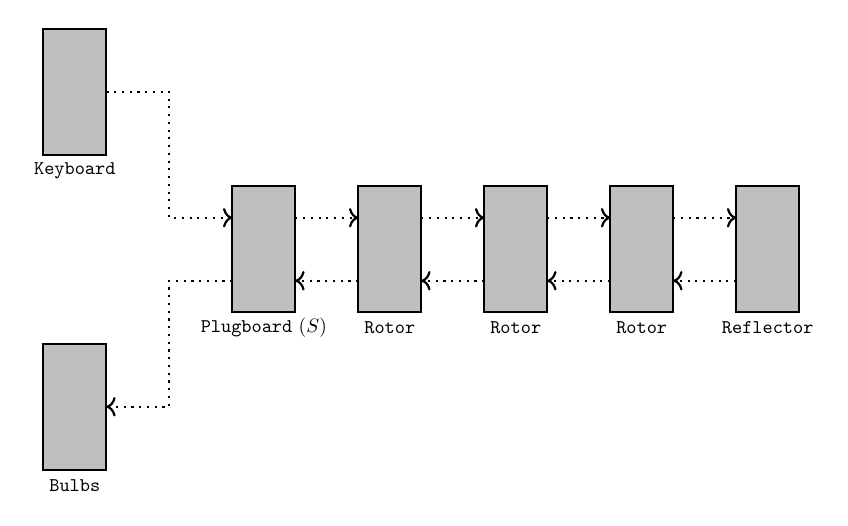
\begin{tikzpicture}[thick, scale=0.4, every node/.style={scale=0.7}]
				\draw[fill=lightgray] (0+5-14, 0+2+5) rectangle (2+5-14,4+2+5) node[midway] {};
				\node at (0+5+1-14, 0+2-0.5+5) {\texttt{Keyboard}};

				\draw[fill=lightgray] (0+5-14, 0+2-5) rectangle (2+5-14,4+2-5) node[midway] {};
				\node at (0+5+1-14, 0+2-0.5-5) {\texttt{Bulbs}};

				\draw[fill=lightgray] (0+5-8, 0+2) rectangle (2+5-8,4+2) node[midway] {};
				\node at (0+5+1-8, 0+2-0.5) {\texttt{Plugboard} ($S$)};

				\draw[fill=lightgray] (0+5, 0+2) rectangle (2+5,4+2) node[midway] {};
				\node at (0+5+1, 0+2-0.5) {\texttt{Rotor}};

				\draw[fill=lightgray] (0+5+4, 0+2) rectangle (2+5+4,4+2) node[midway] {};
				\node at (0+5+1+4, 0+2-0.5) {\texttt{Rotor}};

				\draw[fill=lightgray] (0+5+8, 0+2) rectangle (2+5+8,4+2) node[midway] {};
				\node at (0+5+1+8, 0+2-0.5) {\texttt{Reflector}};

				\draw[fill=lightgray] (0+5-4, 0+2) rectangle (2+5-4,4+2) node[midway] {};
				\node at (0+5+1-4, 0+2-0.5) {\texttt{Rotor}};

				\draw[->,dotted] (0+5-14+2, 0+2+5+2) -- (0+5-10, 0+2+5+2)
				-- (0+5-10, 0+2+5-2) -- (0+5-8, 0+2+5-2);

				\draw[->,dotted] (0+5-6, 0+2+5-2) -- (0+5-4, 0+2+5-2);
				\draw[->,dotted] (0+5-2, 0+2+5-2) -- (0+5, 0+2+5-2);
				\draw[->,dotted] (0+5+2, 0+2+5-2) -- (0+5+4, 0+2+5-2);
				\draw[->,dotted] (0+5+6, 0+2+5-2) -- (0+5+8, 0+2+5-2);

				\draw[->,dotted] (0+5+8, 0+2+5-4) -- (0+5+6, 0+2+5-4);
				\draw[->,dotted] (0+5+4, 0+2+5-4) -- (0+5+2, 0+2+5-4);
				\draw[->,dotted] (0+5, 0+2+5-4) -- (0+5-2, 0+2+5-4);
				\draw[->,dotted] (0+5-4, 0+2+5-4) -- (0+5-6, 0+2+5-4);

				\draw[->,dotted]  (0+5-8, 0+2+5-4) -- (0+5-10, 0+2+5-4)
				-- (0+5-10, 0+2+5-8) -- (0+5-14+2, 0+2+5-8) ;


			\end{tikzpicture}
		}
	\end{center}
    \end{tcolorbox}

\begin{tcolorbox}[colback=white!95!gray, colframe=black!75, boxrule=0.8pt, arc=4pt, width=\textwidth,  title=Enigma Key Sheet, ]
    	\begin{center}
		\begin{figure}[H]
			\begin{center}
				\resizebox{0.98\textwidth}{!}{
					\begin{tabular}{|c|c|c|c|}
						\hline
						\textbf{\emph{\texttt{Datum}}}        &
						\textbf{\emph{\texttt{Walzenlage}}}   &
						\textbf{\emph{\texttt{Ringstellung}}} &
						\textbf{\emph{\texttt{Steckerverbindungen}}}                                                                            \\
						% \textbf{\emph{\texttt{Grundstellung}}}
						% \\
						\hline
						\texttt{31.}                          & \texttt{IV V I}    & \texttt{21 15 16} & \texttt{KL IT FQ HY XC NP VZ JB SE OG} %                                          & \texttt{VAR}
						\\
						\texttt{30.}                          & \texttt{IV II III} & \texttt{26 14 11} & \texttt{ZN YO QB ER DK XU GP TV SJ LM} %                                          & \texttt{PAQ}
						\\
						\texttt{29.}                          & \texttt{II V IV}   & \texttt{19 09 24} & \texttt{ZU HL CQ WM OA PY EB TR DN VI} %                                         & \texttt{ZJB}
						\\
						$\vdots$                              & $\vdots$
						                                      & $\vdots$           & $\vdots$                                                   \\
						\hline
					\end{tabular}}
			\end{center}
		\end{figure}
	\end{center}
    \end{tcolorbox}
    \text{}\\\\\\\\\\\\\\\\\\\\\\\\\large\textbf{Plaintext Attack}
    \\\centerline{\rule{15cm}{0.4pt}}

\begin{figure}[H]
\begin{center}
\begin{tcolorbox}[colback=white!95!gray, colframe=black!75, boxrule=0.8pt, arc=4pt, width=0.4\textwidth,  title=Plaintext Analysis Definitions, ]
    \begin{center}
        $\pi_i = S^{-1}\overline{\pi_i}S$\\
        \vspace{1.5em}

        $\pi \coloneq \pi_{3}\pi_2\pi_1$\\[1ex]
        $\overline{\pi} \coloneq \overline{\pi_{3}\pi_2\pi_1}$
    \end{center}
\end{tcolorbox}
\end{center}
\end{figure}

\begin{tcolorbox}[colback=white!95!gray, colframe=black!75, boxrule=0.8pt, arc=4pt, width=\textwidth, title=Plaintext to Bombe Wiring, ]
\begin{figure}[H]
  \centering
  \begin{minipage}[t]{0.48\textwidth}
    \centering
    \fbox{%
      \begin{minipage}{\textwidth}
	\begin{center}
    \vspace{2.1em}
		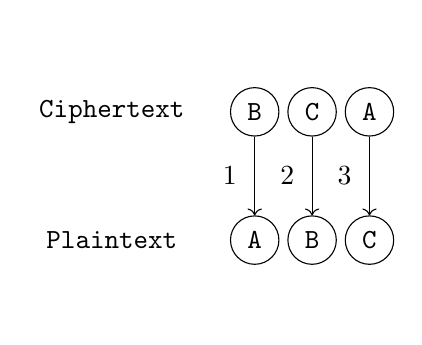
\begin{tikzpicture}[node distance=1cm, every node/.style={draw,
						circle, minimum height=0.1cm, minimum width=0.1cm}]

			% Centering the diagram
			\node (a1) [] {\texttt{B}};
			\node (a2) [right=0.1cm of a1] {\texttt{C}};
			\node (a3) [right=0.1cm of a2] {\texttt{A}};

			% Nodes for ciphertext
			\node (x1) [below=1cm of a1] {\texttt{A}};
			\node (x2) [below=1cm of a2] {\texttt{B}};
			\node (x3) [below=1cm of a3] {\texttt{C}};

			% Arrows for mapping
			\draw[->] (a1) -- (x1) node[midway, left, draw=none, fill=none] {1};
			\draw[->] (a2) -- (x2) node[midway, left, draw=none, fill=none] {2};
			\draw[->] (a3) -- (x3) node[midway, left, draw=none, fill=none] {3};

                 \node[draw=none] at ([xshift=-1.5cm]a1.west) {\texttt{Ciphertext }};
                 \node[draw=none] at ([xshift=-1.5cm]x1.west) {\texttt{Plaintext  }};

		\end{tikzpicture}
        \vspace{2.1em}
	\end{center}
      \end{minipage}%
    }
  \end{minipage}
  \hfill
  \begin{minipage}[t]{0.48\textwidth}
    \centering
    \fbox{%
      \begin{minipage}{\textwidth}
    	\begin{center}
        \scalebox{1.3}{
		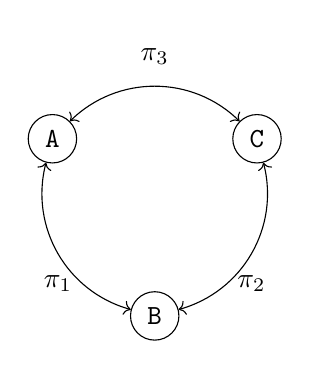
\begin{tikzpicture}[node distance=1cm, every node/.style={draw,
						circle, minimum height=0.1cm, minimum width=0.1cm}]
			\node (A) at (270-120:1.5) {$\texttt{A}$};
			\node (B) at (270:1.5) {$\texttt{B}$};
			\node (C) at (270+120:1.5) {$\texttt{C}$};

			\draw[<->, bend right=45] (A) to node[midway, draw=none, below] {$\pi_1$} (B);
			\draw[<->, bend right=45] (B) to node[midway, draw=none, below] {$\pi_2$} (C);
			\draw[<->, bend right=45] (C) to node[midway, draw=none, above] {$\pi_{3}$} (A);

		\end{tikzpicture}}
	\end{center}
      \end{minipage}%
    }
  \end{minipage}

  \vspace{0.5cm}

  \begin{minipage}[t]{0.48\textwidth}
    \centering
    \fbox{%
      \begin{minipage}{\textwidth}
      \begin{center}
            \begin{tikzpicture}[node distance=1cm, 
              every node/.style={minimum size=0.6cm},
              round/.style={draw, circle, minimum size=0.6cm},
              box/.style={draw, rectangle, minimum width=0.8cm, minimum height=0.6cm}
            ]
              % Main triangle nodes
              \node[round] (A) at (150:2cm) {\texttt{A}};
              \node[round] (B) at (270:2cm) {\texttt{?}};
              \node[round] (C) at (30:2cm) {\texttt{?}};
            
              \node[box, rotate=172-90, fill=lightgray] (PreA) at (172:2cm) {$S^$};
              \node[box, rotate=126.5-90, fill=lightgray] (PostA) at (126.5:2cm) {$S^{-1}$};
              % Arcs between main triangle nodes
              \draw[<->, bend right=43] (PreA) to node[midway, left] {$\overline\pi_1$} (B);
              \draw[<->, bend right=50] (B) to node[midway, right] {$\overline\pi_2$} (C);
              \draw[<->, bend right=42] (C) to node[midway, above] {$\overline\pi_3$} (PostA);
                % Boxes before and after A (along the same radial line)
            
            \end{tikzpicture}
            \end{center}
      \end{minipage}%
    }
  \end{minipage}
  \hfill
  \begin{minipage}[t]{0.48\textwidth}
    \centering
    \fbox{%
      \begin{minipage}{\textwidth}
	\begin{center}
		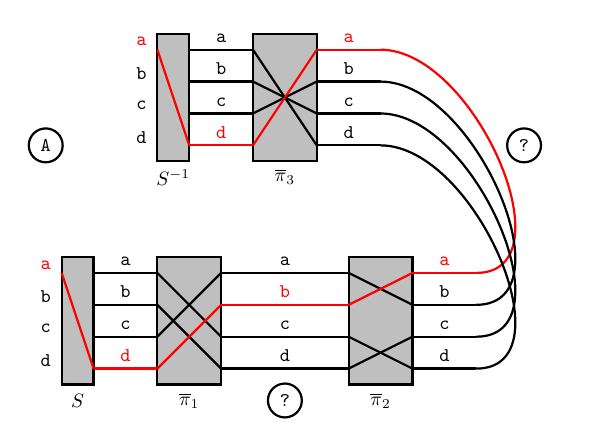
\begin{tikzpicture}[thick, scale=0.405, every node/.style={scale=0.7}]
			% Draw the box
			\draw[fill=lightgray] (2,-1.5) rectangle (4,2.5) node[midway] {};

			\node at (3, -2) {$\overline\pi_{3}$};

            \draw[fill=lightgray] (2-3,-1.5) rectangle (4-4,2.5) node[midway] {};
			\node at (3-3.5, -2) {$S^{-1}$};

            \node[text=red] (Plain) at (2-3-0.5, 2+0.25) {\texttt{a}};
            \node (Plain) at (2-3-0.5, 2+0.25-1) {\texttt{b}};
            \node (Plain) at (2-3-0.5, 2+0.25-2) {\texttt{c}};
            \node (Plain) at (2-3-0.5, 2+0.25-3) {\texttt{d}};

			% Draw the wires entering the box
			\draw[-] (0, 2) -- (2, 2) node[midway, above] {\texttt{a}};
			\draw[-] (0, 1) -- (2, 1) node[midway, above] {\texttt{b}};
			\draw[-] (0, 0) -- (2, 0) node[midway, above] {\texttt{c}};
			\draw[-, red] (0,-1) -- (2,-1) node[midway, above] {\texttt{d}};
            \draw[-, red] (2-3,2) -- (3-3,-1) node[midway, above] {};

			% Draw the wires exiting the box with crossed mappings
			\draw[-, red] (4, 2) -- (6,2) node[midway, above] {\texttt{a}};
			\draw[-] (4, 1) -- (6, 1) node[midway, above] {\texttt{b}};
			\draw[-] (4, 0) -- (6, 0) node[midway, above] {\texttt{c}};
			\draw[-] (4,-1) -- (6, -1) node[midway, above] {\texttt{d}};

			% Draw the lines inside the box to represent the mapping
			\draw[-] (2, 2) -- (4,-1);
			\draw[-] (2, 1) -- (4, 0);
			\draw[-] (2, 0) -- (4, 1);
			\draw[-, red] (2,-1) -- (4, 2);

			% \draw[-] (0-3, 2-7) to[out=180, in=180] (0, 2) node[midway, above] {};
			% \draw[-] (0-3, 1-7) to[out=180, in=180] (0, 1) node[midway, above] {};
			% \draw[-] (0-3, 0-7) to[out=180, in=180] (0, 0) node[midway, above] {};
			% \draw[-] (0-3, -1-7) to[out=180, in=180] (0, -1) node[midway, above] {};

			\draw[-, red] (6+3, 2-7) to[out=360, in=360] (6, 2) node[midway, above] {};
			\draw[-] (6+3, 1-7) to[out=360, in=360] (6, 1) node[midway, above] {};
			\draw[-] (6+3, 0-7) to[out=360, in=360] (6, 0) node[midway, above] {};
			\draw[-] (6+3, -1-7) to[out=360, in=360] (6, -1) node[midway, above] {};

			\draw[fill=lightgray] (2-3,-1.5-7) rectangle (4-3,2.5-7) node[midway] {};

			\node at (3-3, -2-7) {$\overline\pi_1$};

            \draw[fill=lightgray] (2-3-3,-1.5-7) rectangle (4-4-3,2.5-7) node[midway] {};
			\node at (3-3.5-3, -2-7) {$S$};

			% Draw the wires entering the box
			\draw[-] (0-3, 2-7) -- (2-3, 2-7) node[midway, above] {\texttt{a}};
			\draw[-] (0-3, 1-7) -- (2-3, 1-7) node[midway, above] {\texttt{b}};
			\draw[-] (0-3, 0-7) -- (2-3, 0-7) node[midway, above] {\texttt{c}};
			\draw[-, red] (0-3,-1-7) -- (2-3,-1-7) node[midway, above] {\texttt{d}};

			% Draw the wires exiting the box
			\draw[-] (4-3, 2-7) -- (6-3,2-7) node[right, above] {\texttt{a}};
			\draw[-, red] (4-3, 1-7) -- (6-3, 1-7) node[right, above] {\texttt{b}};
			\draw[-] (4-3, 0-7) -- (6-3, 0-7) node[right, above] {\texttt{c}};
			\draw[-] (4-3,-1-7) -- (6-3, -1-7) node[right, above] {\texttt{d}};

			% Draw the lines inside the box to represent the mapping
            \draw[-, red] (2-3-3, 2-7) -- (4-3-4, -1-7);
			\draw[-] (2-3, 2-7) -- (4-3, 0-7);
			\draw[-] (2-3, 1-7) -- (4-3, -1-7);
			\draw[-] (2-3, 0-7) -- (4-3, 2-7);
			\draw[-, red] (2-3,-1-7) -- (4-3, 1-7);

            \node[text=red] (Plain) at (2-3-3-0.5, 2-7+0.25) {\texttt{a}};
            \node (Plain) at (2-3-3-0.5, 2-7+0.25-1) {\texttt{b}};
            \node (Plain) at (2-3-3-0.5, 2-7+0.25-2) {\texttt{c}};
            \node (Plain) at (2-3-3-0.5, 2-7+0.25-3) {\texttt{d}};

			\draw[fill=lightgray] (2+3,-1.5-7) rectangle (4+3,2.5-7) node[midway] {};

			\node at (3+3, -2-7) {$\overline\pi_2$};

			% Draw the wires entering the box
			\draw[-] (0+3, 2-7) -- (2+3, 2-7) node[midway, above] {};
			\draw[-, red] (0+3, 1-7) -- (2+3, 1-7) node[midway, above] {};
			\draw[-] (0+3, 0-7) -- (2+3, 0-7) node[midway, above] {};
			\draw[-] (0+3,-1-7) -- (2+3,-1-7) node[midway, above] {};

			% Draw the wires exiting the box
			\draw[-, red] (4+3, 2-7) -- (6+3,2-7) node[midway, above] {\texttt{a}};
			\draw[-] (4+3, 1-7) -- (6+3, 1-7) node[midway, above] {\texttt{b}};
			\draw[-] (4+3, 0-7) -- (6+3, 0-7) node[midway, above] {\texttt{c}};
			\draw[-] (4+3,-1-7) -- (6+3, -1-7) node[midway, above] {\texttt{d}};

			\draw[-] (2+3, 2-7) -- (4+3, 1-7);
			\draw[-, red] (2+3, 1-7) -- (4+3, 2-7);
			\draw[-] (2+3, 0-7) -- (4+3, -1-7);
			\draw[-] (2+3,-1-7) -- (4+3, 0-7);

			\node[draw,circle] at (-4.5, -1) {\texttt{A}};
			\node[draw,circle] at (3, -9) {\texttt{?}};
			\node[draw,circle] at (10.5, -1) {\texttt{?}};

		\end{tikzpicture}
	\end{center}
      \end{minipage}%
    }
  \end{minipage}
\end{figure}
\end{tcolorbox}
    \text{}\\\\\\\large\textbf{Dixon's Theorem and Generalization}
    \\\centerline{\rule{15cm}{0.4pt}}


    \vspace{2em}
    \begin{tcolorbox}[colback=white!95!gray, colframe=black!75, boxrule=0.8pt, arc=4pt, width=\textwidth, title=Dixon's Theorem (1969), ]
    \begin{center}
		\emph{Given two uniformly random permutations $\sigma$ and $\tau$ in $S_n$, the
		probability that form a transitive subgroup of $S_n$ is}
		\begin{align*}
			t_n = 1-\frac{1}{n!}\sum_{1^{\ell_1}\dots n^{\ell_n} \ne n^1}\prod_{i=1}^n{\frac{(i!t_{i})^{\ell_i}}{\ell_i!}}
		\end{align*}
		\emph{where $t_i$ is the probability that two random permutations in
		$S_i$ form a transitive subgroup.}
    \end{center}
    \end{tcolorbox}
    \begin{tcolorbox}[colback=white!95!gray, colframe=black!75, boxrule=0.8pt, arc=4pt, width=\textwidth, title=\textsc{GeneralDixons} Algorithm, ]
    \begin{center}
    	\scalebox{0.82}{
		\begin{minipage}{\linewidth}
			\begin{algorithmic}[1]
				\Function{GeneralDixons}{$p_1$, $p_2$, $n$}
				\Comment{$p_1$, $p_2$: partition of $n$ representing each permutation's cycle types}


				\Comment{$n$: size of the symmetric group}
				\If{$|p_1| = 1$ \textbf{or} $|p_2| = 1$}
				\State \Return $1.0$
				\EndIf
				\State $S \gets$ (number of permutation pairs with cycle types $p_1$ and $p_2$)
				\State $R \gets S$
				\For{integer partition $\nu = (\nu_1, \nu_2, \dots, \nu_k)$ of $n$}
				\If{$|\nu| = 1$} \State \textbf{continue} \EndIf
				\State $C_1, C_2 \gets$ (partitions of $p_1$, $p_2$ whose sums are $\nu_i$s)
				\State $T \gets 0$
				\For{$(c_1, c_2)$ in $C_1 \times C_2$}
				\State $P \gets 1$
				\For{$i = 1$ to $|\nu|$}
				\State $P \gets P \times$ (number of permutation pairs with cycle types $c_1[i]$ and $c_2[i]$)
				\State $P \gets P \times$ \Call{GeneralDixons}{$c_1[i]$, $c_2[i]$, $\nu_i$}
				\EndFor
				\State $T \gets T + P$
				\EndFor
				\State $R \gets R - T \times$ (number of set partitions of $\mathbb{N}_n$ of type $\nu$)
				\EndFor
				\State \Return $R / S$
				\EndFunction
			\end{algorithmic}
		\end{minipage}}
    \end{center}
    \end{tcolorbox}

    \text{}\large\textbf{Results}
    \\\centerline{\rule{15cm}{0.4pt}}

    \begin{tcolorbox}[colback=white!95!gray, colframe=black!75, boxrule=0.8pt, arc=4pt, width=\textwidth, title=Single Loop Calculation and Simulation ]
        	\begin{table}[H]
		\centering
		\begin{tabular}{|c|c|c|}
			\hline
			{\bf{ $\ell$ }} & {\bf{ Expected Stops }} & {\bf{ Simulated Stops }} \\
			\hline
			2               & 17576.00                & $17576.00 \pm 0.00$      \\
			\hline
			3               & 16246.63                & $16243.78 \pm 6.91$      \\
			\hline
			4               & 17576.00                & $17576.00 \pm 0.00$      \\
			\hline
			5               & 16224.88                & $16220.57 \pm 6.66$      \\
			\hline
			6               & 17576.00                & $17576.00 \pm 0.00$      \\
			\hline
			7               & 16222.69                & $16224.37 \pm 6.63$      \\
			\hline
			8               & 17576.00                & $17576.00 \pm 0.00$      \\
			\hline
			9               & 16223.75                & $16227.80 \pm 6.92$      \\
			\hline
			10              & 17576.00                & $17576.00 \pm 0.00$      \\
			\hline
			11              & 16224.53                & $16228.59 \pm 6.95$      \\
			\hline
			12              & 17576.00                & $17576.00 \pm 0.00$      \\
			\hline
		\end{tabular}
	\end{table}
    \end{tcolorbox}
    \vspace{18em}
    \begin{tcolorbox}[colback=white!95!gray, colframe=black!75, boxrule=0.8pt, arc=4pt, width=\textwidth, title=Two Loop Calculation ]
    	\begin{table}[H]
		\centering
		\begin{adjustbox}{max width=\textwidth,max height=2\textheight}
\begin{tabular}{|c|c|c|c|c|c|c|c|c|c|c|c|}
  \hline
  & 2       & 3       & 4       & 5       & 6       & 7       & 8       & 9       & 10      & 11      & 12      \\
  \hline
  2 & \textbf{781.69} & \textbf{749.40} & \textbf{750.42} & \textbf{751.24} & \textbf{750.81} & \textbf{750.08} & \textbf{750.78} & 750.25 & \textbf{750.05} & \textbf{750.24} & \textbf{750.13} \\
  \hline
  3 &               & \textbf{704.13} & \textbf{705.75} & \textbf{706.53} & \textbf{706.12} & \textbf{705.39} & \textbf{706.07} & \textbf{705.55} & \textbf{705.35} & \textbf{705.56} & \textbf{705.40} \\
  \hline
  4 &               &               & \textbf{707.42} & \textbf{708.20} & \textbf{707.79} & \textbf{707.05} & \textbf{707.74} & \textbf{707.21} & \textbf{707.02} & \textbf{707.22} & 707.07 \\
  \hline
  5 &               &               &               & \textbf{708.98} & \textbf{708.57} & \textbf{707.83} & \textbf{708.51} & 707.99 & \textbf{707.80} & \textbf{708.00} & 707.84 \\
  \hline
  6 &               &               &               &               & \textbf{708.16} & \textbf{707.42} & \textbf{708.11} & \textbf{707.59} & \textbf{707.39} & \textbf{707.59} & \textbf{707.44} \\
  \hline
  7 &               &               &               &               &               & \textbf{706.68} & \textbf{707.37} & \textbf{706.85} & \textbf{706.65} & \textbf{706.85} & 706.70 \\
  \hline
  8 &               &               &               &               &               &               & \textbf{708.05} & \textbf{707.53} & \textbf{707.33} & \textbf{707.54} & \textbf{707.38} \\
  \hline
  9 &               &               &               &               &               &               &               & \textbf{707.01} & \textbf{706.81} & \textbf{707.02} & \textbf{706.86} \\
  \hline
  10 &              &               &               &               &               &               &               &               & 706.62 & \textbf{706.82} & \textbf{706.67} \\
  \hline
  11 &              &               &               &               &               &               &               &               &               & \textbf{707.02} & \textbf{706.87} \\
  \hline
  12 &              &               &               &               &               &               &               &               &               &               & \textbf{706.72} \\
  \hline
\end{tabular}

		\end{adjustbox}
		\begin{center}Values within the $95\%$ margin of
			error of the following table are noted in
			\textbf{bold}.\end{center}
	\end{table}
    \end{tcolorbox}
      \begin{tcolorbox}[colback=white!95!gray, colframe=black!75, boxrule=0.8pt, arc=4pt, width=\textwidth, title=Two Loop Simulation ]
    \renewcommand{\arraystretch}{1.5}
    
	\begin{table}[H]
		\centering
		\small
		\begin{adjustbox}{max width=\textwidth}
			\begin{tabular}{|c|c|c|c|c|c|c|c|c|c|c|c|}
				\hline
				                  & 2                 & 3                 & 4                 & 5                 & 6                 & 7                 & 8                 & 9                 & 10                & 11                & 12                \\
				\hline
				2                 & $781.08 \pm 4.99$ & $749.89 \pm 3.58$ & $752.43 \pm 3.43$ &
				$748.28 \pm 3.46$ & $749.09 \pm 3.42$ & $751.22 \pm 3.47$ &
				$749.06 \pm 3.42$ & $753.89 \pm 3.58$ & $749.75 \pm 3.56$ &
				$750.87 \pm 3.49$ & $750.22 \pm 3.57$                                                                                                                                                                                                         \\
				\hline
				3                 &                   & $704.02 \pm 1.73$ & $705.49 \pm 1.75$ & $706.84 \pm 1.69$
				                  & $706.50 \pm 1.78$ & $705.45 \pm 1.68$ & $705.42 \pm 1.70$ &
				$706.25 \pm 1.69$ & $706.54 \pm 1.69$ & $706.08 \pm 1.62$ &
				$705.98 \pm 1.70$                                                                                                                                                                                                                             \\
				\hline
				4                 &                   &                   & $707.55 \pm 1.63$ & $707.93 \pm 1.59$ & $707.22 \pm
				1.60$             & $706.95 \pm 1.58$ & $707.50 \pm 1.66$ & $708.45 \pm
				1.65$             & $707.32 \pm 1.63$ & $707.85 \pm 1.66$ & $709.15 \pm 1.62$                                                                                                                                                                 \\
				\hline
				5                 &                   &                   &                   & $708.55 \pm 1.65$ & $707.70 \pm 1.61$ & $708.97 \pm
				1.61$             & $707.65 \pm 1.65$ & $706.33 \pm 1.59$ & $707.45 \pm
				1.66$             & $707.84 \pm 1.68$ & $705.78 \pm 1.57$                                                                                                                                                                                     \\
				\hline
				6                 &                   &                   &                   &                   & $706.69 \pm 1.59$ & $706.74 \pm 1.61$ & $706.55 \pm
				1.66$             & $706.21 \pm 1.60$ & $707.41 \pm 1.57$ & $707.38 \pm
				1.62$             & $707.28 \pm 1.66$                                                                                                                                                                                                         \\
				\hline
				7                 &                   &                   &                   &                   &                   & $707.64 \pm 1.61$ & $708.29 \pm 1.56$ & $707.38
				\pm 1.60$         & $708.17 \pm 1.60$ & $705.95 \pm 1.58$ & $708.60 \pm 1.58$                                                                                                                                                                 \\
				\hline
				8                 &                   &                   &                   &                   &                   &                   & $707.48 \pm 1.63$ & $707.15 \pm 1.59$ & $706.82
				\pm 1.66$         & $707.60 \pm 1.61$ & $706.73 \pm 1.61$                                                                                                                                                                                     \\
				\hline
				9                 &                   &                   &                   &                   &                   &                   &                   & $706.91 \pm 1.64$ & $708.12 \pm 1.64$ &
				$706.56 \pm 1.57$ & $707.28 \pm 1.60$                                                                                                                                                                                                         \\
				\hline
				10                &                   &                   &                   &                   &                   &                   &                   &                   & $708.33 \pm 1.62$ & $707.54 \pm 1.58$ &
				$707.88 \pm 1.61$                                                                                                                                                                                                                             \\
				\hline
				11                &                   &                   &                   &                   &                   &                   &                   &                   &                   & $707.23 \pm 1.63$ & $707.18 \pm 1.62$ \\
				\hline
				12                &                   &                   &                   &                   &                   &                   &                   &                   &                   &                   & $708.22 \pm 1.60$ \\
				\hline
			\end{tabular}
		\end{adjustbox}
	\end{table}
    \end{tcolorbox}
\end{document}
